\documentclass{article}
\usepackage[utf8]{inputenc}
\usepackage{graphicx}
\graphicspath{{Images/}}
\usepackage{amsmath}
\usepackage{parskip}
\usepackage[a4paper, total={6in, 8in}]{geometry}
\title{A Look At Lagrangian Mechanics}
\author{Freddie Floydd}

\setlength{\parskip}{10pt}
\setlength{\parindent}{0pt}

\begin{document}
\maketitle

\section{Introduction}
Lagrangian Mechanics is a branch of classical mechanics which uses energies rather than forces to produce equations of motion. This is often superior to Newtonian Mechanics when dealing with complex situations, as it is easier to consider an object's potential and kinetic energies, which are both scalars, than to work out the directions and magnitudes of the forces acting on it. By using the Lagrangian of a system we can obtain a set of equations for the second derivatives of the system's variables in terms of the variables themselves and the first derivatives, the equations of motion. By solving the equations of motion for the system either analytically or via numerical methods we can model how the system evolves over time. In general, the Lagrangian of a system is defined as
$$ L \equiv T - V \, ,$$
where T = Sum of Kinetic Energies and V = Sum of Potential Energies.

This definition may seem arbitrary but it leads to a very useful result, called the Euler-Lagrange equation:
$$ \frac{d}{dt} \left( \frac{\partial L}{\partial \dot{x}} \right) = \frac{\partial L}{\partial x} \, .$$   
The proof of this result is frankly over my head mathematically, but that will not stop me from using it to have some fun with mechanics. For those interested it depends on the principle of stationary action.

\section{Applying the Lagrangian}
To see this equation in action, let's look at the simple situation of a pendulum.

\begin{figure}[ht]
\centering
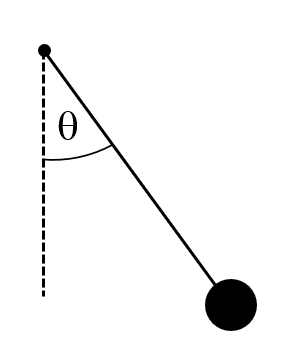
\includegraphics[width=4cm]{Lagrangian_Pendulum.jpg}
\caption{A simple pendulum}
\end{figure}

We can see in Fig.1 that the potential and kinetic energies are:
\begin{align*}
    V &= mgr \thinspace (1 - \cos{\theta}) \\
    T &= \frac{1}{2} mr^2\dot{\theta}
\end{align*}
So the Lagrangian is
$$ L = \frac{1}{2}mr^2 \dot{\theta} + mgr \thinspace(\cos{\theta} - 1) \, .$$
From this we can differentiate with respect to \(\theta\) and \(\dot{\theta}\) to obtain the following expressions:
\begin{align*}
    \frac{\partial L}{\partial \theta} &= -mgr\sin{\theta} \\
    \frac{\partial L}{\partial \dot{\theta}} &= mr^2 \dot{\theta} \\
    \frac{d}{dt} \left( \frac{\partial L}{\partial \dot{\theta}} \right) &= mr^2\ddot{\theta}  
\end{align*}
Using the Euler-Lagrange equation from above, we get
$$ \ddot{\theta} = -\frac{g\sin{\theta}}{r} \, .$$ 
This is the equation of motion for a simple pendulum which can be obtained through Newtonian mechanics, via resolving forces on the pendulum bob for a given angle \(\theta\). A differential equation is very useful for any mechanical system, as it tells us how a system will change over time given a set of initial conditions, for example the initial speed at which the pendulum is projected and its initial angle. Note that for small values of \(\theta\) we can use a small angle approximation here to give
$$ \ddot{\theta} = - \frac{g}{r} \theta \, ,$$
which is by definition simple harmonic motion. This method is much simpler than the Newtonian approach however, as we do not have to deal with the directions of forces acting on the pendulum bob. This allows us to look at much more complex situations, such as a double pendulum.

\section{More Complex Situations}
In more complex situations there are often more variables to keep track of than just a single angle. We are able to form differential equations for each variable by performing the same process as above on the Lagrangian for each of the variables, allowing us to model the situation with a system of multiple differential equations, which can be solved simultaneously. While these systems are very rarely analytically solvable, we can employ computers to find numerical solutions. (I have written a few programs modelling complex mechanical situations, based off differential equations formed using the Lagrangian method, which can be found on Github.) Now, as promised, let's look at something more interesting.

\begin{figure}[ht!]
\centering
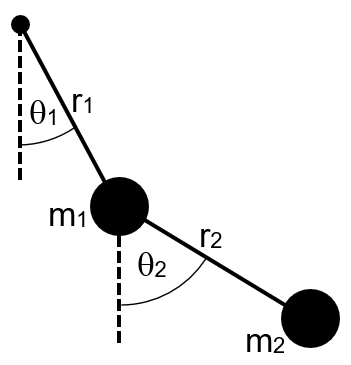
\includegraphics[width=4cm]{Lagrangian_Double_Pendulum.jpg}
\caption{A double pendulum}
\end{figure}
A double pendulum, while at face value not appearing much more complex than a single pendulum, is a completely different scenario in that as well as gravity providing a constant downward force on each of the bobs, the motion of each bob will exert a force on the other, making the system extremely chaotic. 

Our first step is to identify the Cartesian coordinates of each mass.
\begin{align*}
    (x,\thinspace y)_{m_{1}} &= (r_{1}\sin{\theta_1} ,\thinspace -r_{1}\cos{\theta_{1}}) \\
    (x,\thinspace y)_{m_{2}} &= (r_{1}\sin{\theta_1} + r_{2}\sin{\theta_2},\thinspace -r_{1}\cos{\theta_{1}} - r_{2}\cos{\theta_{2}} )
\end{align*}
We can now differentiate each of these positions with respect to time to obtain the velocity of each mass.
\begin{align*}
   (\dot{x},\thinspace \dot{y})_{m_{1}} &= (r_{1}\dot{\theta}_{1}\cos{\theta_1} ,\thinspace r_{1}\dot{\theta}_{1}\sin{\theta_{1}}) \\
   (\dot{x},\thinspace \dot{y})_{m_{2}} &= (r_{1}\dot{\theta}_{1}\cos{\theta_1} + r_{2}\dot{\theta}_{2}\cos{\theta_{2}},\thinspace r_{1}\dot{\theta}_{1}\sin{\theta_{1}} + r_{2}\dot{\theta}_{2}\sin{\theta_{2}}) 
\end{align*}
We now have all we need to make expressions for the potential and kinetic energy of the system. As we know,
\begin{align*}
    V &= mgh \\
    T &= \frac{mv^2}{2} \, .
\end{align*}
From these we can form the Lagrangian.
\begin{align*}
    V &= -r_{1}m_{1}g\cos{\theta_{1}} - m_{2}g \thinspace (r_{1}\cos{\theta_{1}} + r_{2}\cos{\theta_{2}}) \\
    T &= \frac{1}{2} r_{1}^2 m_{1} \dot{\theta}_{1}^2 + \frac{1}{2}m_{2}(r_{1}^2 \dot{\theta}_{1}^2 + r_{2}^2 \dot{\theta}_{2}^2 + 2r_{1}r_{2}\dot{\theta}_{1}\dot{\theta}_{2}\cos{(\theta_{1}-\theta_{2})})
\end{align*}
\begin{align*}
 L = &\frac{1}{2} r_{1}^2 m_{1} \dot{\theta}_{1}^2 + \frac{1}{2}m_{2}(r_{1}^2 \dot{\theta}_{1}^2 + r_{2}^2 \dot{\theta}_{2}^2 + 2r_{1}r_{2}\dot{\theta}_{1}\dot{\theta}_{2}\cos{(\theta_{1}-\theta_{2})}) \\
&+ r_{1}m_{1}g\cos{\theta_{1}} + m_{2}g \thinspace (r_{1}\cos{\theta_{1}} + r_{2}\cos{\theta_{2}})
\end{align*}
 We can now find a number of derivatives, which can be used to form a pair of coupled differential equations.
\begin{align*}
    \frac{\partial L}{\partial \dot{\theta}_{1}} &= r_{1}^2 \dot{\theta}_{1} (m_{1} + m_{2})+ r_{1}r_{2}m_{2} \dot{\theta}_{2}\cos{(\theta_{1} - \theta_{2})} \\
    \frac{\partial L}{\partial \theta_{1}} &= - r_{1}g\sin{\theta_1}(m_{1} + m_{2}) - r_{1}r_{2}m_{2}\dot{\theta}_{1}\dot{\theta}_{2}\sin{(\theta_{1}-\theta_{2})} \\
    \frac{d}{dt} \frac{\partial L}{\partial \dot{\theta}_{1}} &= r_{1}^2 \ddot{\theta}_{1} (m_{1} + m_{2})+ r_{1}r_{2}m_{2} \ddot{\theta}_{2}\cos{(\theta_{1} - \theta_{2})} - r_{1}r_{2}m_{2} \dot{\theta}_{2}(\dot{\theta}_{1} - \dot{\theta}_{2})\sin{(\theta_{1} - \theta_{2})} \\
    \frac{\partial L}{\partial \dot{\theta}_{2}} &= r_{2}^2 m_{2}\dot{\theta}_{2}  + r_{1}r_{2}m_{2} \dot{\theta}_{1}\cos{(\theta_{1} - \theta_{2})} \\
    \frac{\partial L}{\partial \theta_{2}} &= - r_{2}m_{2}g\sin{\theta_1} +  r_{1}r_{2}m_{2}\dot{\theta}_{1}\dot{\theta}_{2}\sin{(\theta_{1}-\theta_{2})} \\
    \frac{d}{dt} \frac{\partial L}{\partial \dot{\theta}_{2}} &= r_{1}^2 \ddot{\theta}_{1} (m_{1} + m_{2})+ r_{1}r_{2}m_{2} \ddot{\theta}_{2}\cos{(\theta_{1} - \theta_{2})} - r_{1}r_{2}m_{2} \dot{\theta}_{2}(\dot{\theta}_{1} - \dot{\theta}_{2})\sin{(\theta_{1} - \theta_{2})}
\end{align*}
 Using the derivatives we can form the differential equations for the system.
\begin{align*}
r_{1}\ddot{\theta}_{1}(m_{1} + m_{2}) + r_{2}m_{2} \ddot{\theta}_{2}\cos{(\theta_{1} - \theta_{2})} + r_{2}m_{2}\dot{\theta}_{2}^2\sin{(\theta_{1} - \theta_{2})} &=
- g\sin{\theta_1}(m_{1} + m_{2}) \\
r_{2}\ddot{\theta}_{2} + r_{1} \ddot{\theta}_{1}\cos{(\theta_{1} - \theta_{2})} - r_{1}\dot{\theta}_{1}^2\sin{(\theta_{1} - \theta_{2})} &= - g\sin{\theta_2}
\end{align*}
While these differential equations cannot be solved analytically, we can solve them numerically by rearranging to eliminate \( \ddot{\theta}_{2} \) from the first equation. This gives us an expression for \(\ddot{\theta}_{1}\) in terms of \(\theta_{1}\), \(\theta_{2}\), \(\dot{\theta}_{1}\) and \(\dot{\theta}_{2}\). We can also rearrange to give a similar equation for \(\ddot{\theta}_{2}\). Using these equations we an substitute in values for these variables and obtain an angular acceleration for each of \(\theta_{1}\) and \(\theta_{2}\). We can then add this acceleration to the corresponding angular velocities, and add the angular velocities to the angles. repeating this process millions of times per second will give a very close approximation to how an analytic solution to the equations would behave. To visualize this system I programmed a simulation to model the equations. As can be seen in the trace of the pendulum below, the system is very chaotic.

\begin{figure}[h!]
\centering
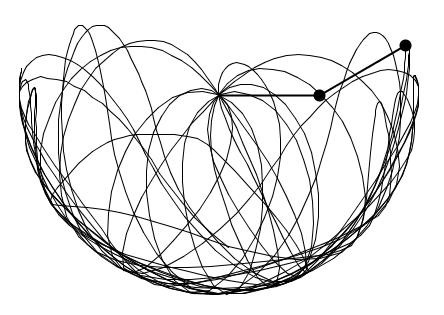
\includegraphics[width=6.25cm]{Double_Pendulum_Trace.jpg}
\caption{The trace of a double pendulum, with the initial conditions shown}
\end{figure}

\section{Taking Things Further}

There are many more situations that can be investigated using Lagrangian mechanics, such as triple (or even more!) pendulums, making special relativistic corrections to systems, or virtually any convoluted mechanics problem you could think of. Below are a number of situations I looked at in addition to those above, with the relevant differential equations describing the systems. I have made simulations of the special relativistic pendulums to illustrate the differences in the system due to the correction at low and high speeds.

\subsection{The Triple Pendulum}

 Despite only having one more bob than a double pendulum, the triple is significantly more complex to model using the Lagrangian, due to having three differential equations to form, and there being more inter-bob forces at play. It is also significantly harder to model computationally, without doing some clever work with matrices, though more will be explained about that later.

\begin{figure}[h!]
\centering
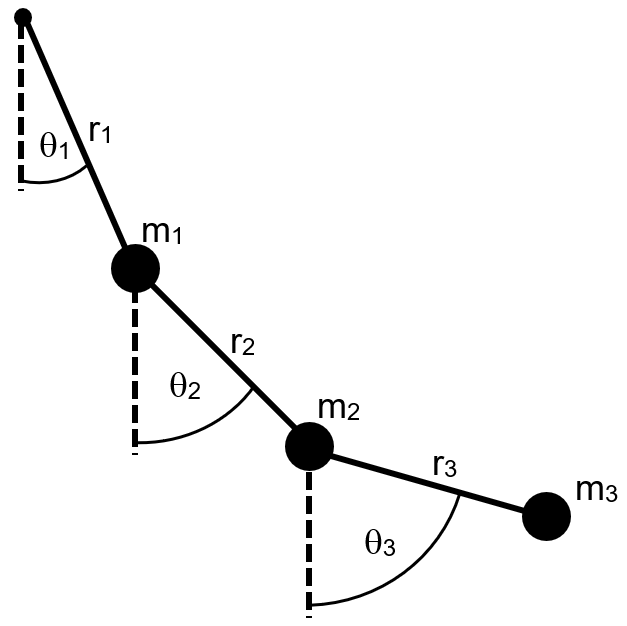
\includegraphics[width=5cm]{Lagrangian_Triple_Pendulum.jpg}
\caption{A triple pendulum}
\end{figure}

The system can be described by the following equations:
\begin{align*}
r_{1}(m_{1} + m_{2} + m_{3}) \ddot{\theta}_{1} &= -g (m_{1} + m_{2} + m_{3}) \sin{\theta_{1}} - r_{2} (m_{2} + m_{3}) \left(\ddot{\theta}_{2} \cos{(\theta_{1} - \theta_{2})} + \dot{\theta}_2^2 \sin{(\theta_{1} - \theta_{2})}\right) \\ &- r_{3} m_{3} \left(\ddot{\theta}_{3} \cos{(\theta_{1} - \theta_{3})} + \dot{\theta}_3^2 \sin{(\theta_{1} - \theta_{3})}\right) \\
r_{2}(m_{2} + m_{3}) \ddot{\theta}_{2} &= -g (m_{2} + m_{3}) \sin{\theta_{2}} - r_{1} (m_{2} + m_{3}) \left(\ddot{\theta}_{1} \cos{(\theta_{2} - \theta_{1})} + \dot{\theta}_1^2 \sin{(\theta_{2} - \theta_{1})}\right) \\ &- r_{3} m_{3} \left(\ddot{\theta}_{3} \cos{(\theta_{2} - \theta_{3})} + \dot{\theta}_3^2 \sin{(\theta_{2} - \theta_{3})}\right) \\
r_{3} \ddot{\theta}_{3} &= -g \sin{\theta_{3}} - r_{1} \left(\ddot{\theta}_{1} \cos{(\theta_{3} - \theta_{1})} + \dot{\theta}_1^2 \sin{(\theta_{3} - \theta_{1})}\right) \\ &- r_{2} \left(\ddot{\theta}_{2} \cos{(\theta_{3} - \theta_{2})} + \dot{\theta}_2^2 \sin{(\theta_{3} - \theta_{2})}\right)
\end{align*}
At this point you may be able to spot a pattern in the equations which was also present in the equations for the double pendulum. It is in fact possible to generalize these equations of motion to larger numbers of pendulums, allowing more complex systems to be modelled without the need to derive the equations of motion by hand each time.

\subsection{Block and Pendulum on a Slope}

This was one of the first problems I attempted to model using the Lagrangian, and is a good one to have a go at yourself should you feel inclined. This is an interesting situation because while looking at this using forces would be very complicated, the Lagrangian approach greatly simplifies it.

\begin{figure}[h!]
\centering
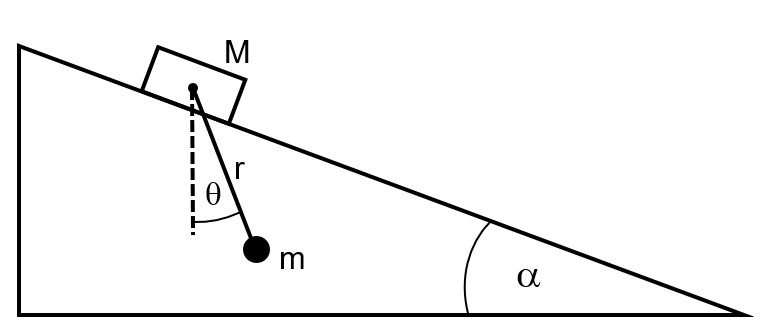
\includegraphics[width=5cm]{Lagrangian_Block_On_Slope.jpg}
\caption{A complex mechanical system}
\end{figure}

 If we take z to be the distance moved down the slope by the block, then the equations of motion for the system are:
\begin{align*}
    (M + m) \ddot{z} + m r \left(\ddot{\theta} \cos{(\theta + \alpha)} - \dot{\theta}^2 \sin{(\theta + \alpha)} \right) &= (M + m) g \sin{\alpha} \\
    r \ddot{\theta} + \ddot{z} \cos{(\theta + \alpha)} &= -g \sin{\theta}
\end{align*}


\subsection{Relativistic Correction for a Single Pendulum}

In a standard single pendulum, the bob will move nowhere near the speed of light, but it is interesting to consider the effects special relativity would have if the speed of light was much lower. Using Special Relativity, we arrive at the following equation for an object's kinetic energy
$$ KE = m_{0} c^2 \left( \frac{1}{\sqrt{1 - \frac{v^2}{c^2}}} - 1 \right) \, ,$$
where \(m_{0} \) is the 'rest mass' of the object, the mass it has when it is not moving, \(v\) is the speed of the object and \(c\) is the speed of light. When  \( v << c\), this expression simplifies to Newtonian KE, but diverges greatly from this as \(v \) approaches \(c \). The differential equation for the relativistic pendulum is similar to the simple one, but has a multiplying factor which reduces the acceleration as the speed of the bob increases.

$$ \ddot{\theta} \left(\gamma ^3 + \frac{3r^2 \dot{\theta}^2}{c^2} \gamma ^5 \right) = -\frac{g}{r} \sin{\theta} $$
\begin{center}
Where \( \gamma = \frac{1}{\sqrt{1 - \frac{r^2 \dot{\theta}^2}{c^2}}} \)
\end{center}

\subsection{Relativistic Correction for a Double Pendulum}

 In the same way the Lagrangian of the double pendulum is significantly harder than that of the single pendulum, applying special relativity to a double pendulum is much, much more complex than any of the previous situations, and is a good way to end this investigation into how far Lagrangian mechanics can be taken. It should be noted that when \( v << c\), these differential equations simplify to the same as those obtained in the earlier derivation. 
\begin{align*}
- (m_{1} + m_{2}) g \sin{\theta_{1}} &=  m_{1} r_{1} \ddot{\theta}_{1} \left( \phi^3 + 3 \phi^5 \big(r_{1} \dot{\theta}_{1} + r_{2} \dot{\theta}_{2} \cos{\alpha} \big) \Big( \frac{ r_{1} \dot{\theta}_{1} + r_{2} \dot{\theta}_{2} \cos{\alpha}}{c^2} \Big) + \frac{3 r_{1}^2 \dot{\theta}_{1}^2 \gamma^5}{c^2} + \gamma^3 \right) \\ &+ m_{2} r_{2} \ddot{\theta}_{2} \left( \phi^3 \cos{\alpha} + 3 \phi^5 \big(r_{1} \dot{\theta}_{1} + r_{2} \dot{\theta}_{2} \cos{\alpha} \big) \Big( \frac{ r_{2} \dot{\theta}_{2} + r_{1} \dot{\theta}_{1} \cos{\alpha}}{c^2} \Big) \right) \\ &+ m_{2} r_{2} \sin{\alpha} \left( \dot{\theta}_{2}^2 \phi^3 + 3 \phi^5 \big(r_{1} \dot{\theta}_{1} + r_{2} \dot{\theta}_{2} \cos{\alpha} \big) \Big( \frac{r_{1} \dot{\theta}_{1} \dot{\theta}_{2} (\dot{\theta}_{2} - \dot{\theta}_{1})}{c^2} \Big) \right) \\ \\
- g \sin{\theta_{2}} &= r_{2} \ddot{\theta}_{2} \left( \phi^3 + 3 \phi^5 \big(r_{2} \dot{\theta}_{2} + r_{1} \dot{\theta}_{1} \cos{\alpha} \big) \Big( \frac{ r_{2} \dot{\theta}_{2} + r_{1} \dot{\theta}_{1} \cos{\alpha}}{c^2} \Big) \right) \\ &+ r_{1} \ddot{\theta}_{1} \left( \phi^3 \cos{\alpha} + 3 \phi^5 \big(r_{2} \dot{\theta}_{2} + r_{1} \dot{\theta}_{1} \cos{\alpha} \big) \Big( \frac{ r_{1} \dot{\theta}_{1} + r_{2} \dot{\theta}_{2} \cos{\alpha}}{c^2} \Big) \right) \\ &- r_{1} \sin{\alpha} \left( \dot{\theta}_{1}^2 \phi^3 - 3 \phi^5 \big(r_{2} \dot{\theta}_{2} + r_{1} \dot{\theta}_{1} \cos{\alpha} \big) \Big( \frac{r_{2} \dot{\theta}_{1} \dot{\theta}_{2} (\dot{\theta}_{2} - \dot{\theta}_{1})}{c^2} \Big) \right)
\end{align*}

\begin{center}
Where \( \gamma = \Big( 1 - \frac{r_{1}^2 \dot{\theta}_{1}^2}{c^2} \Big)^{-\frac{1}{2}} \), \( \phi = \Big( 1 - \frac{r_{1}^2 \dot{\theta}_{1}^2 + r_{2}^2 \dot{\theta}_{2}^2 + 2 r_{1} r_{2} \dot{\theta}_{1} \dot{\theta}_{2} \cos{\alpha}}{c^2} \Big)^{-\frac{1}{2}} \) and \( \alpha = \theta_{1} - \theta_{2} \).
\end{center} 

\section{A Final Look at Pendula}

 If you look carefully at the above equations of motion for the double and triple pendulums, you may spot a pattern. It turns out that we can generalize the equations of motion for an n-bobbed pendulum, and instead of forming a large number of differential equations, each of which must be rearranged to give a given angular acceleration, we can instead form a matrix equation which can be solved to give all the angular accelerations at once. This works because matrices can be used to solve linear systems of equations, and the equations of motion for the system are linear in terms of the angular accelerations. We can feed this matrix equation through a computer program and solve it in a similar manner to how the equations were solved for the double pendulum earlier.

\begin{multline*}
\begin{pmatrix}
a_{1} \cos(\theta_{1} - \theta_{1}) & b_{1} \cos(\theta_{1} - \theta_{2}) & \dots & z_{1} \cos(\theta_{1} - \theta_{n}) \\
a_{2} \cos(\theta_{2} - \theta_{1}) & b_{2} \cos(\theta_{2} - \theta_{2}) & \dots & z_{2} \cos(\theta_{2} - \theta_{n}) \\
\vdots & \vdots & \ddots & \vdots \\
a_{n} \cos(\theta_{n} - \theta_{1}) & b_{n} \cos(\theta_{n} - \theta_{2}) & \dots & z_{n} \cos(\theta_{n} - \theta_{n})
\end{pmatrix}
\begin{pmatrix}
r_{1} \ddot{\theta}_{1} \\ r_{2} \ddot{\theta}_{2} \\ \vdots \\  r_{n} \ddot{\theta}_{n}
\end{pmatrix}
= \\ -g
\begin{pmatrix}
a_{1} \sin(\theta_{1}) \\ b_{2} \sin(\theta_{2}) \\ \vdots \\ z_{n} \sin(\theta_{2})
\end{pmatrix}
 - 
\begin{pmatrix}
a_{1} \sin(\theta_{1} - \theta_{1}) & b_{1} \sin(\theta_{1} - \theta_{2}) & \dots & z_{1} \sin(\theta_{1} - \theta_{n}) \\
a_{2} \sin(\theta_{2} - \theta_{1}) & b_{2} \sin(\theta_{2} - \theta_{2}) & \dots & z_{2} \sin(\theta_{2} - \theta_{n}) \\
\vdots & \vdots & \ddots & \vdots \\
a_{n} \sin(\theta_{n} - \theta_{1}) & b_{n} \sin(\theta_{n} - \theta_{2}) & \dots & z_{n} \sin(\theta_{n} - \theta_{n})
\end{pmatrix}
\begin{pmatrix}
r_{1} \dot{\theta}_{1}^2 \\ r_{2} \dot{\theta}_{2}^2 \\ \vdots \\  r_{n} \dot{\theta}_{n}^2
\end{pmatrix}
\end{multline*}
 All of the values \( a_{1} \dots z_{n} \) are simply sums of masses which follow a simple pattern, while the equation can be rearranged to give an expression for the vector containing the angular accelerations. By solving this equation numerically we can make very accurate models of n pendulum systems.

\begin{figure}[htb]
     \centering
     \fbox{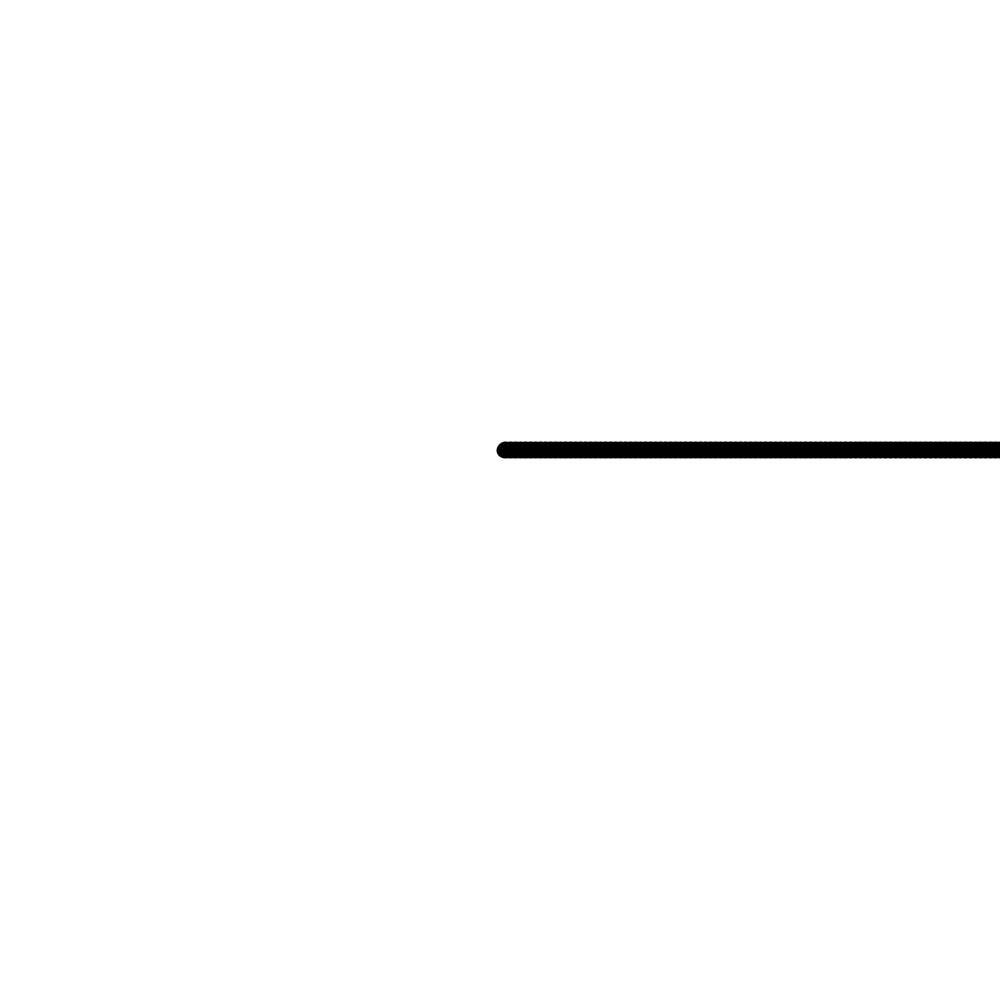
\includegraphics[width=.16\linewidth]{frame2-00001.png}}
     \fbox{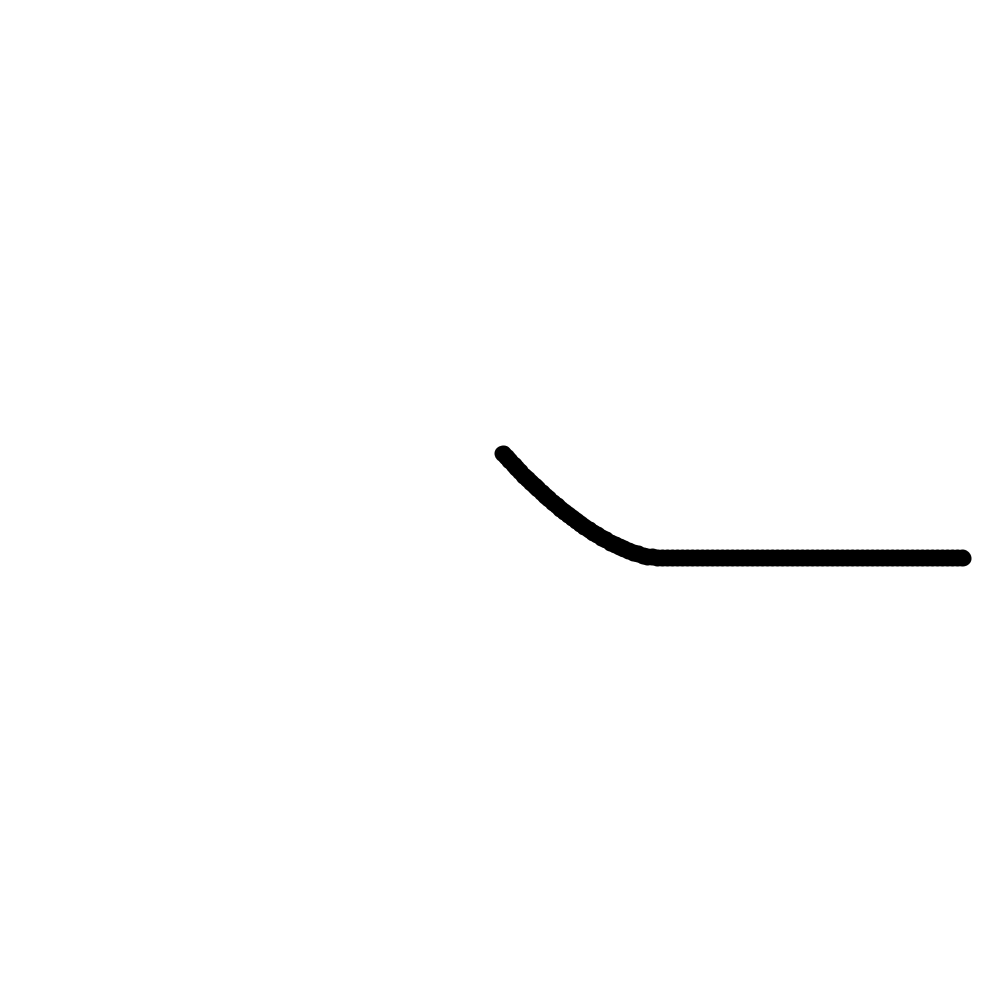
\includegraphics[width=.16\linewidth]{frame2-00022.png}}
     \fbox{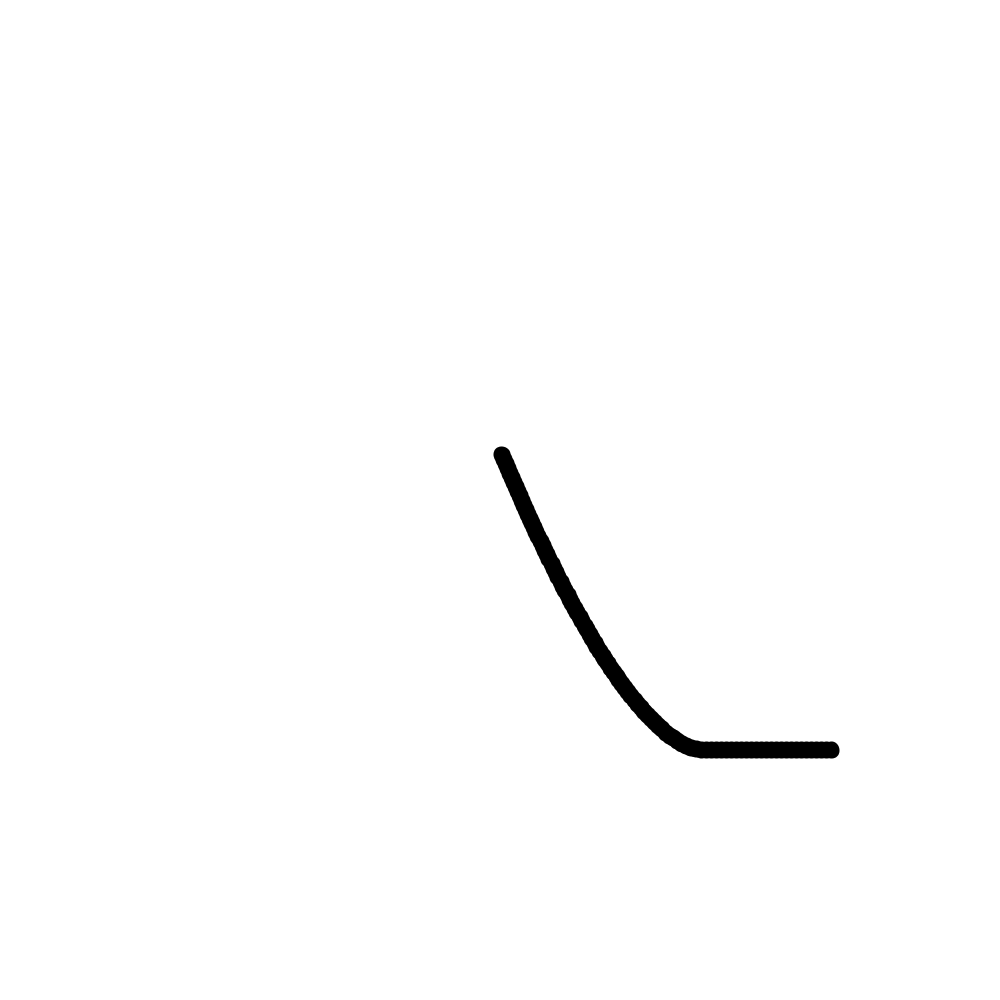
\includegraphics[width=.16\linewidth]{frame2-00036.png}}
     \fbox{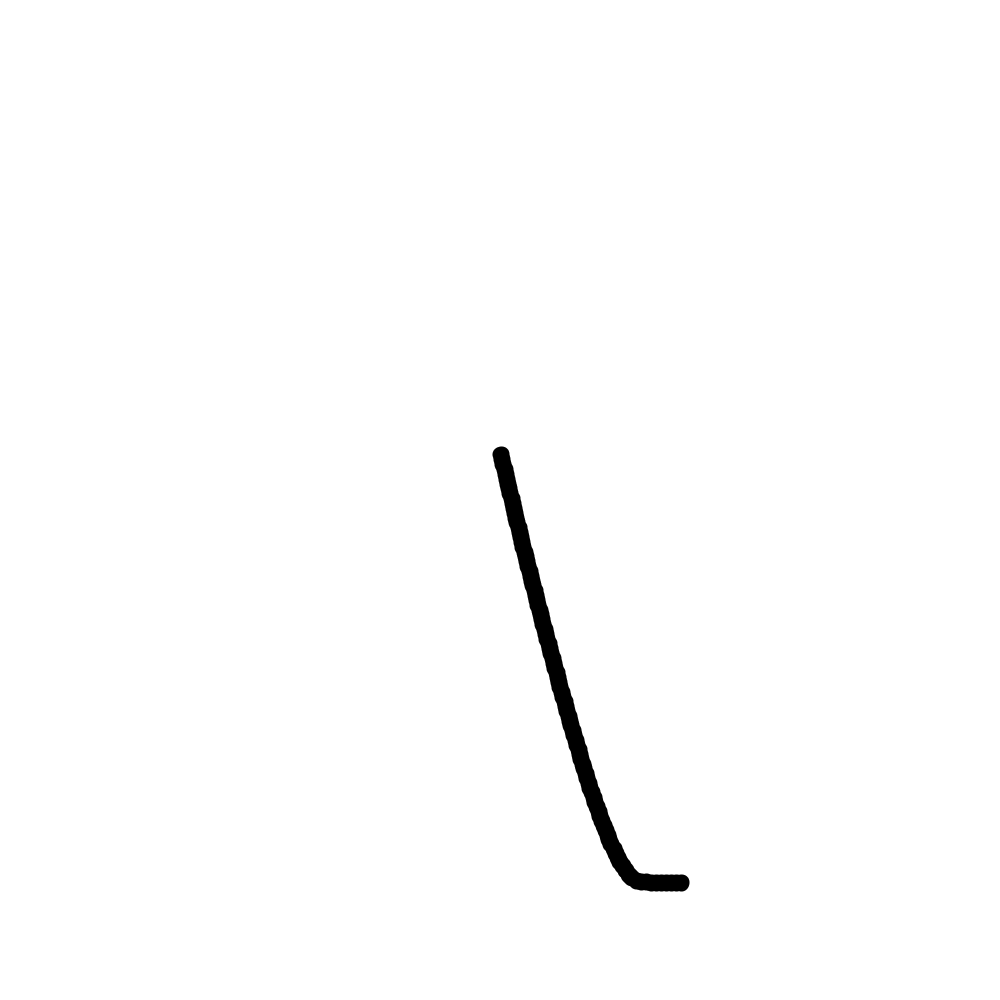
\includegraphics[width=.16\linewidth]{frame2-00043.png}}
     \fbox{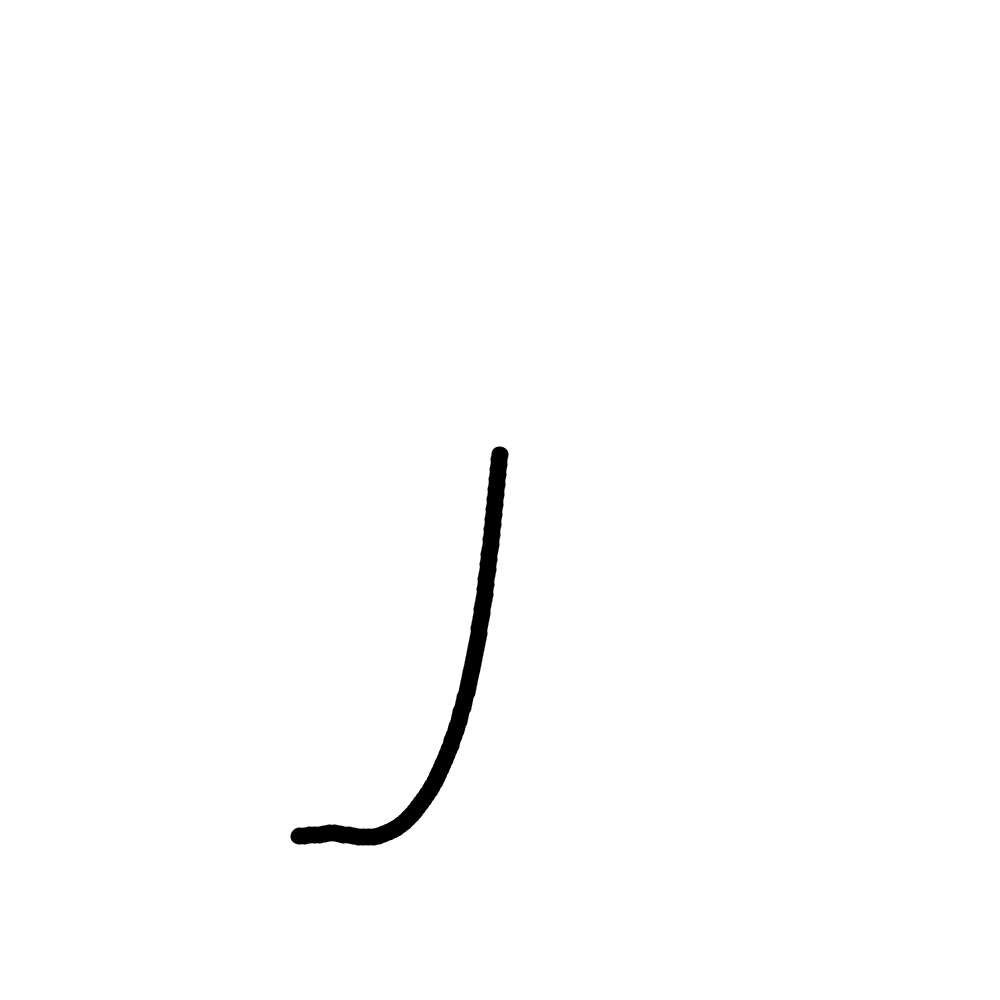
\includegraphics[width=.16\linewidth]{frame2-00054.png}}
     \fbox{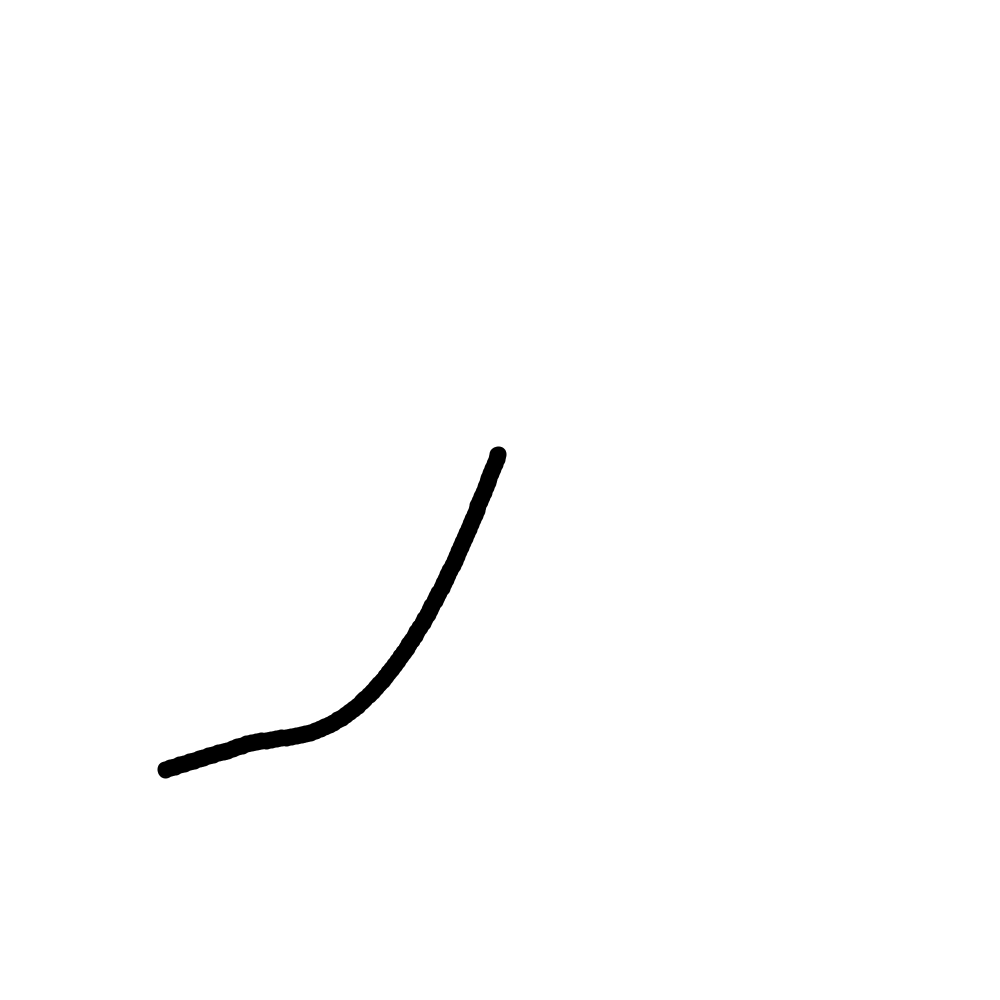
\includegraphics[width=.16\linewidth]{frame2-00061.png}}
     \fbox{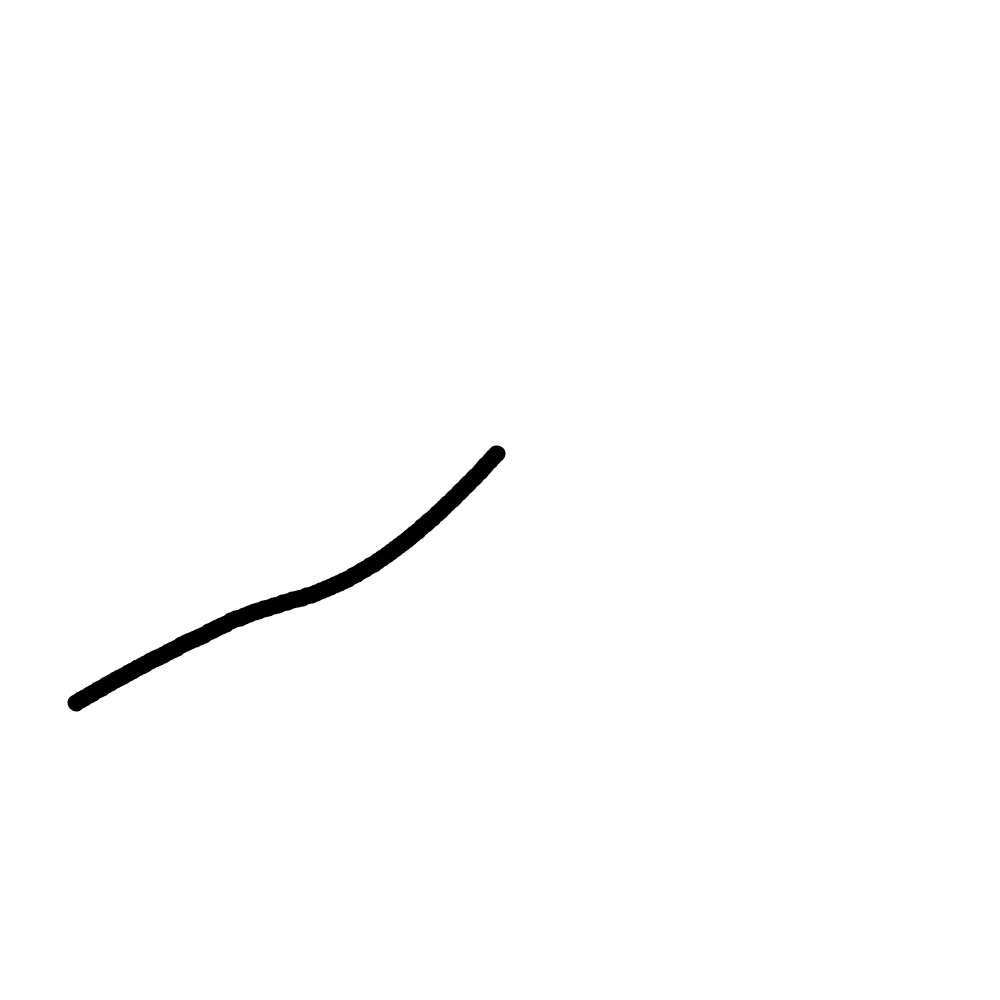
\includegraphics[width=.16\linewidth]{frame2-00069.png}}
     \fbox{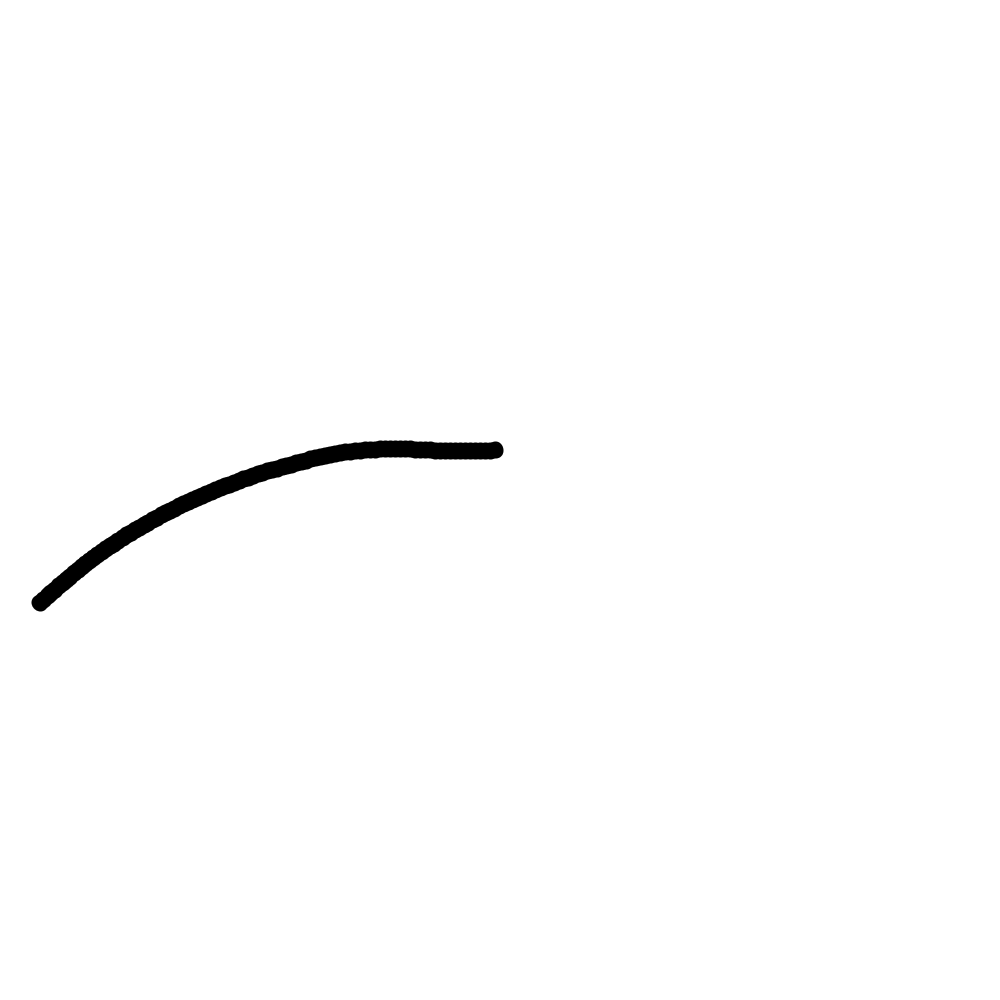
\includegraphics[width=.16\linewidth]{frame2-00081.png}}
     \fbox{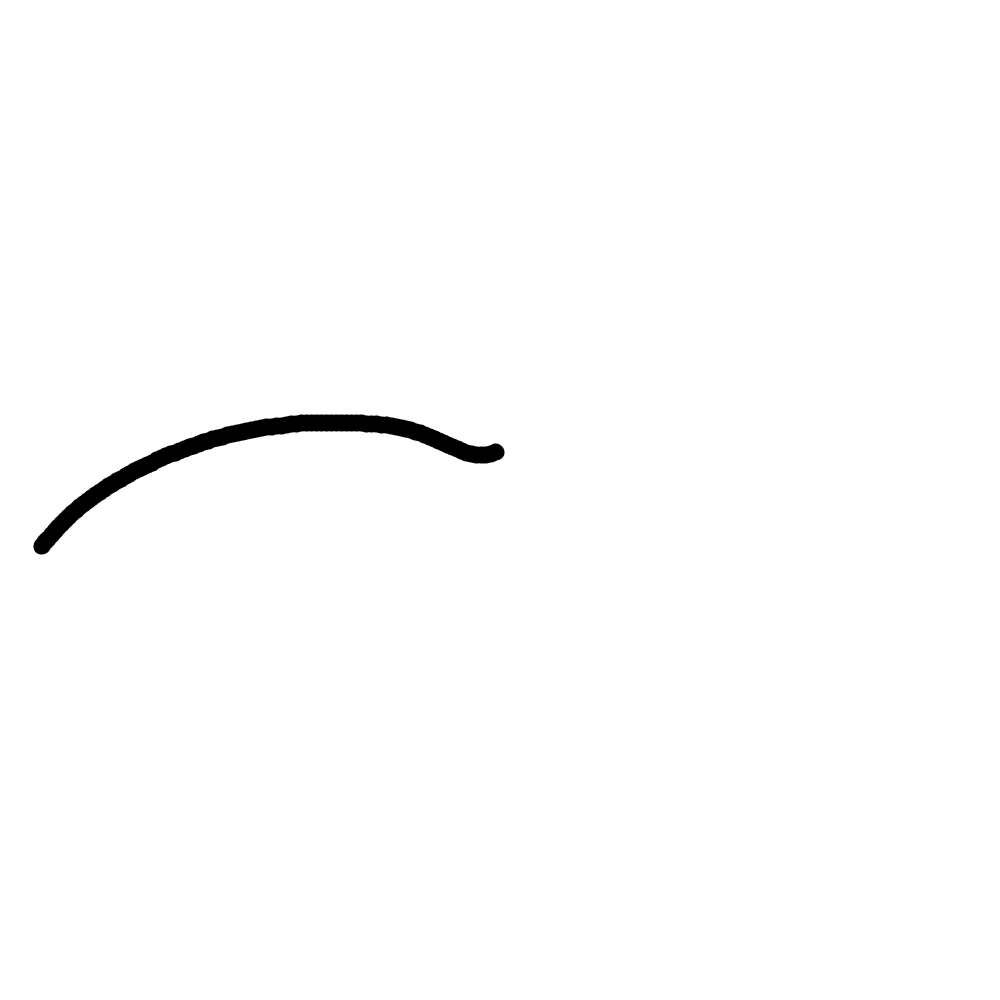
\includegraphics[width=.16\linewidth]{frame2-00092.png}}
     \fbox{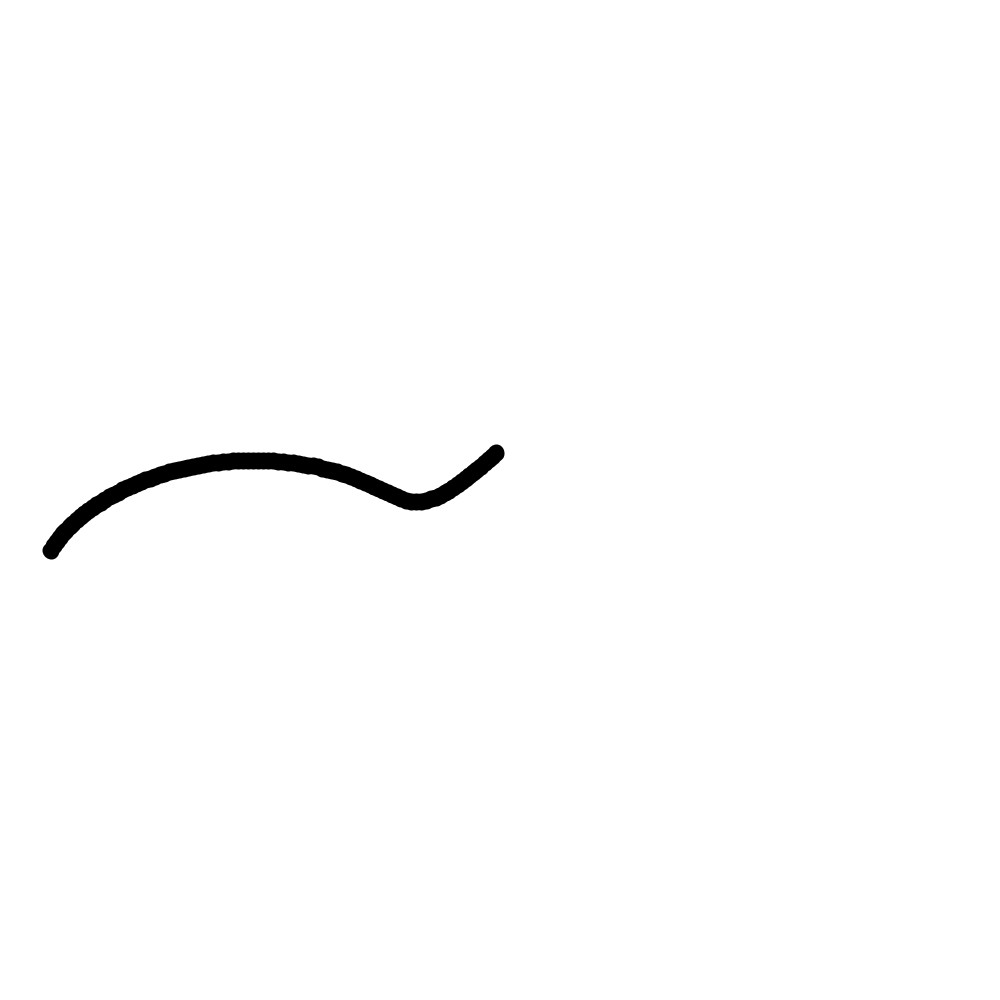
\includegraphics[width=.16\linewidth]{frame2-00106.png}}
     \fbox{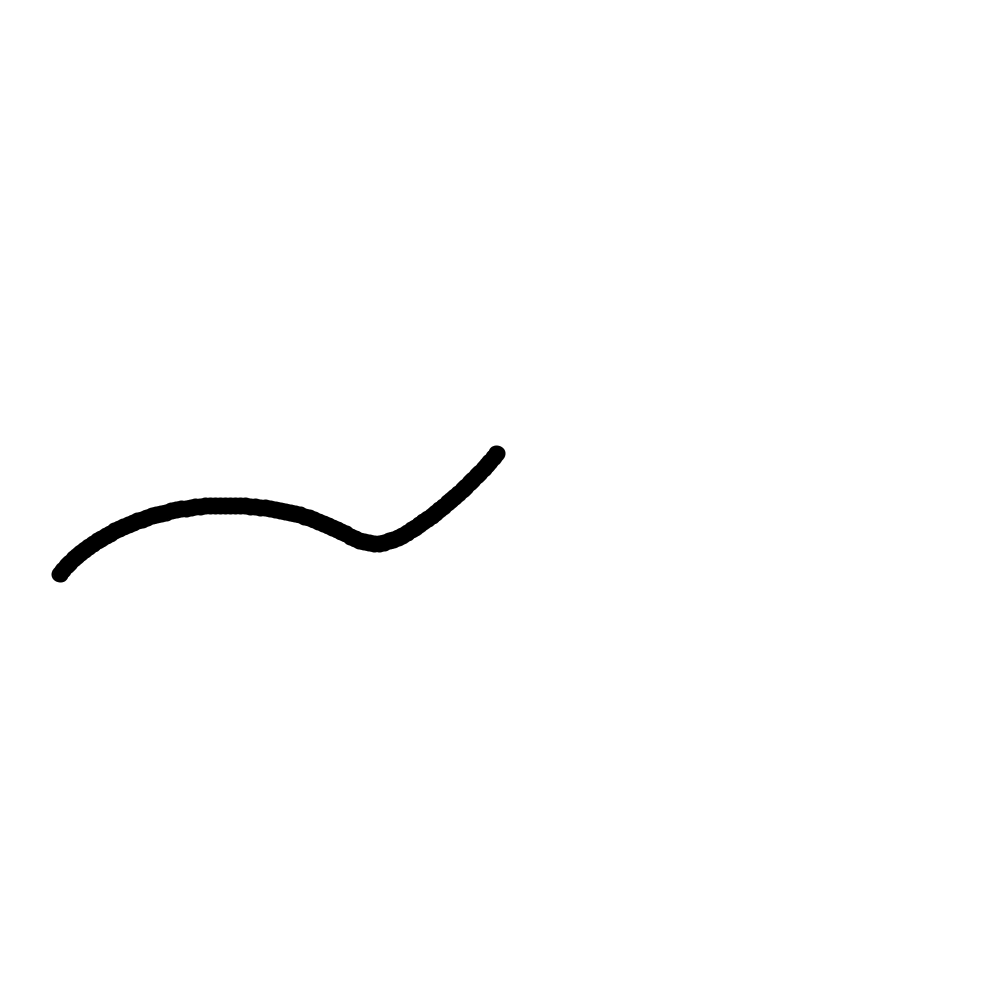
\includegraphics[width=.16\linewidth]{frame2-00112.png}}
     \fbox{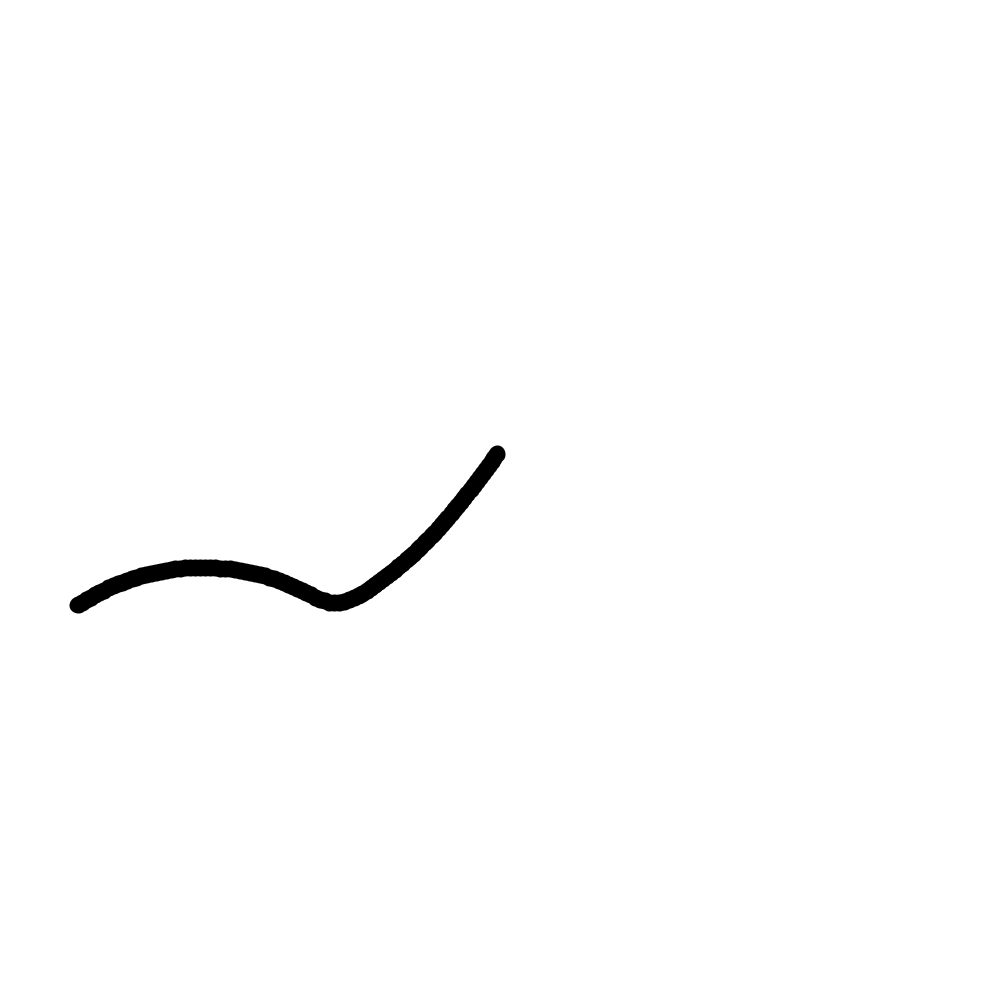
\includegraphics[width=.16\linewidth]{frame2-00118.png}}
     \fbox{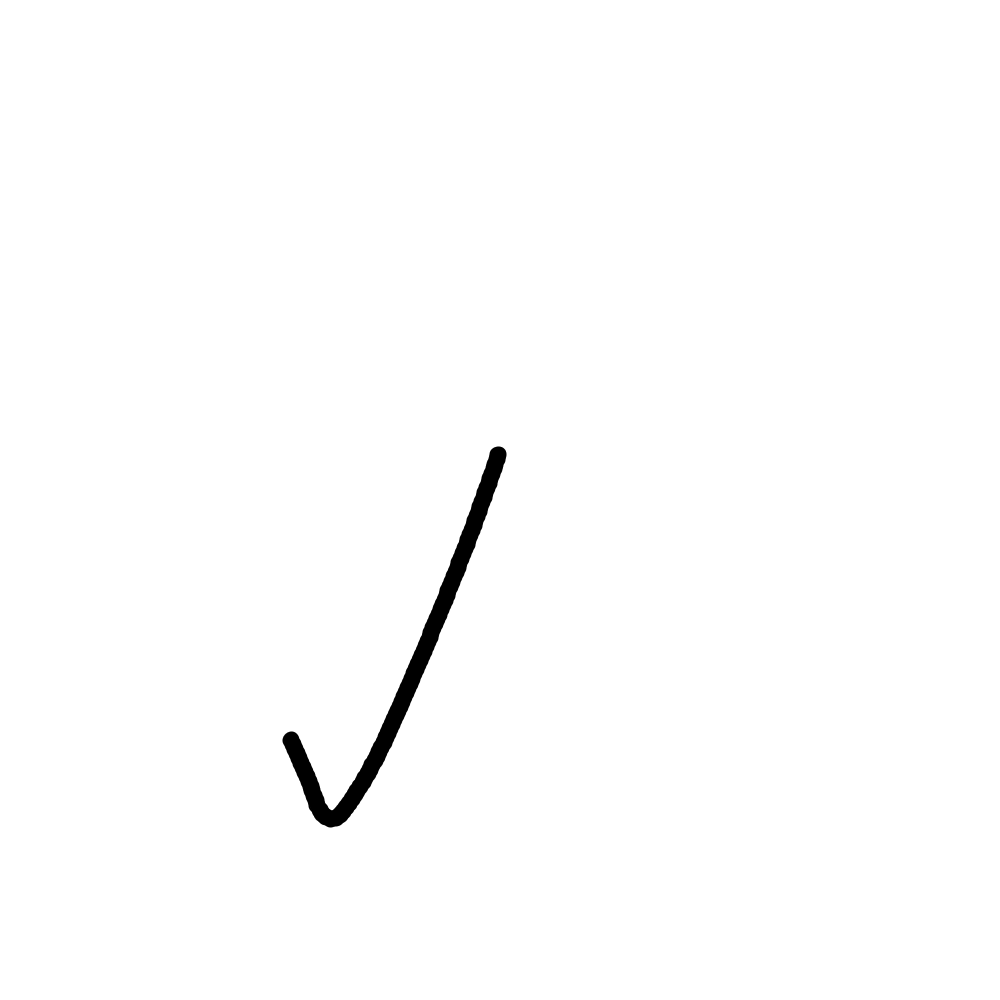
\includegraphics[width=.16\linewidth]{frame2-00133.png}}
     \fbox{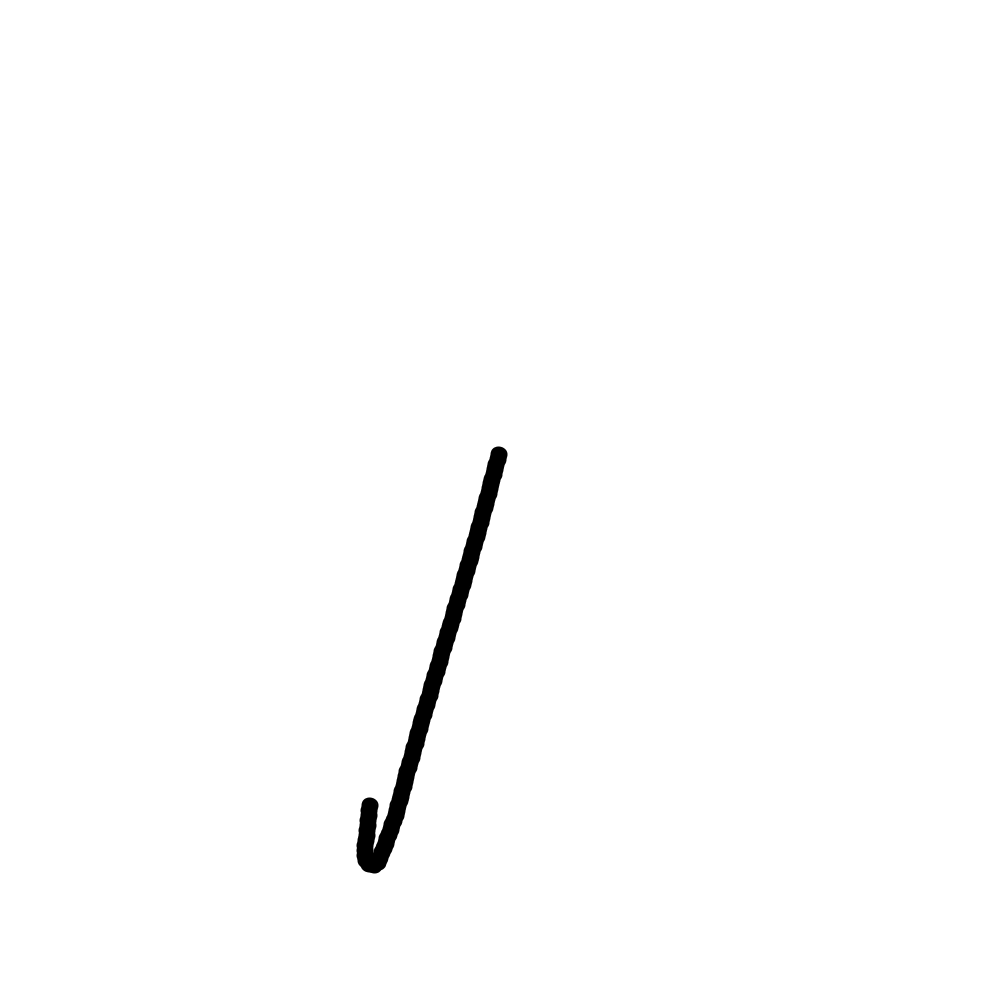
\includegraphics[width=.16\linewidth]{frame2-00136.png}}
     \fbox{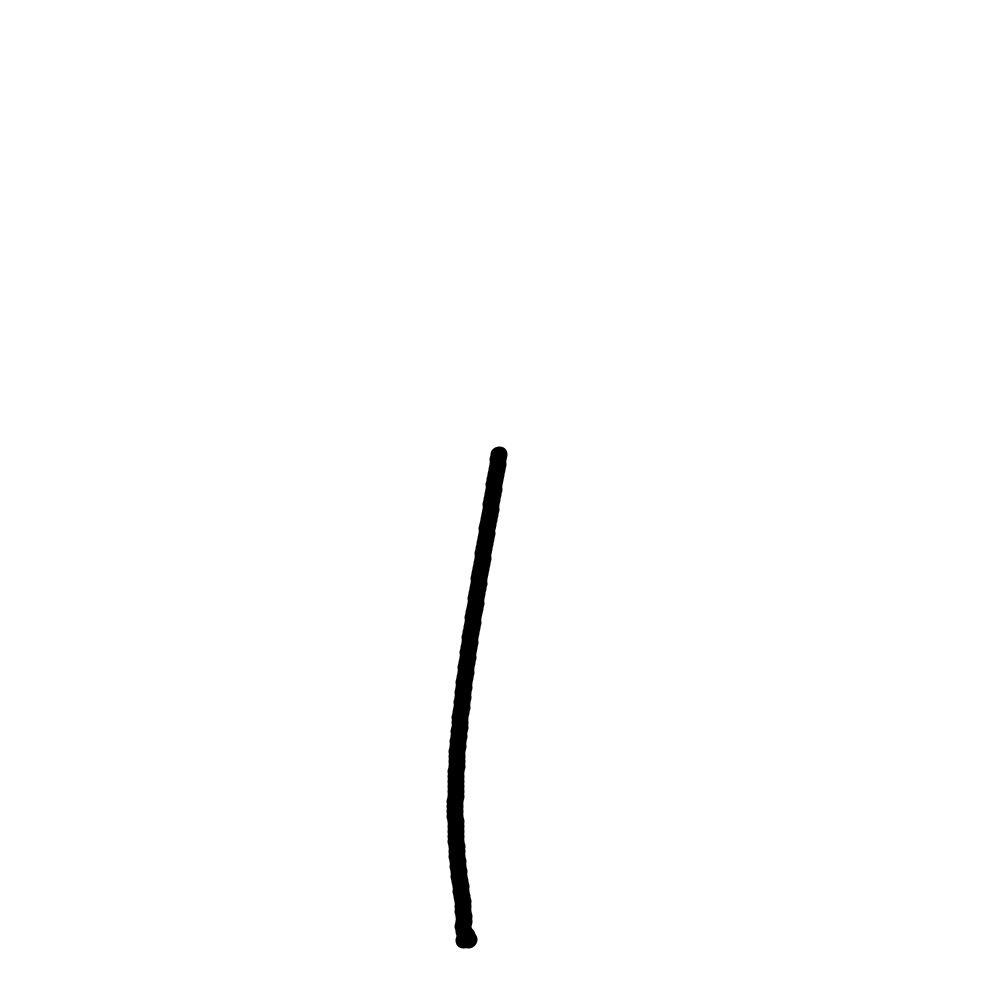
\includegraphics[width=.16\linewidth]{frame2-00140.png}}
     \caption{Frames from a rendering of a 100 pendulum system, giving an approximate simulation of a rope}
\end{figure}
\section{Conclusion}
From the examples above, I hope it is clear that Lagrangian Mechanics is a very powerful tool when looking at challenging mechanical situations. The ability to form equations of motion is always valuable, whether they are solvable analytically or not. An interesting extension of Lagrangian Mechanics is Hamiltonian Mechanics, where instead of obtaining a single second order DE, two first order DEs are obtained. The Hamiltonian also looks at momentum and position, instead of position and velocity, and therefore is a more general form of the Lagrangian. Both Lagrangian and Hamiltonian mechanics are used in very high level physics, such as in quantum mechanics where the action of one object will affect all others, creating an extremely complex system which could not be modelled with forces.

\end{document};
